%-----------------------------------------------------------------------------%
\chapter{Introduction}
%-----------------------------------------------------------------------------%
%-----------------------------------------------------------------------------%

%-----------------------------------------------------------------------------%
\section{Overview and Trends}
WSNs are wireless networks consisting of spatially distributed autonomous nodes using sensors to monitor physical conditions \cite{6188353, 7299315, LONG201739, Pham2017}.  A rapidly increasing range of WSNs are now applied in health monitoring and, military surveillance, and they are especially widely used in industrial systems \cite{Quang2012, 7273816}. With the emergence of the Internet of Things (IoT), WSN becomes more exciting, and until today the unstoppable evolution can be witnessed \cite{6714496, 7120024}. Through IoT, anything or anyone can be connected anytime and anywhere. Recently, Industrial and IP-enabled low-power wireless technologies are emerging, and resulting Industrial IoT (IIoT). When IIoT network is controlled correctly \cite{998012, KIM20031301}, it provides reliability, scalability, interoperability, and economic benefits due to eliminating much wire. 

Steel mills, oil refineries, and offshore drilling platforms implement complex industrial processes, which require tight control and a scalable diagnostic transport. Thousands of sensing points are used to report temperature, pressure, and tank fill levels to an industrial process control center. This center, either in an automated way or through human intervention, uses that information to control an actuator, start a new production stage, scheduled maintenance, or trigger an alarm. Communication between sensors, actuators, and the control center is done through an industrial network. This class of network needs to offer ultra-high reliability while operating reliably in harsh environments. Network failures can have catastrophic consequences and are therefore not an option. To gain higher security and reliability, an industrial network is classically partitioned in a hierarchical manner per the Purdue Enterprise Reference Architecture (PERA), using different technologies at each level, and wireless networks are used at the last hop(s) to the field devices. Industrial networking technology has developed over the last 40 years to satisfy those requirements. A dominant industrial standard is HART \cite{6728782}, a set of standards covering the protocol, connectors, and wires interconnecting the different networked elements. Depending on the safety regulations in use, the price of drawing cables across an industrial plant can run from \$100s/ft to \$1,000s/ft. Planning, installing, and maintaining these cables represent a significant portion of the cost of ownership of such a wired industrial network. As detailed in this article, advances in reliable wireless technology enable low-power wireless networks to exhibit 99.999\% end-to-end reliability and a decade of battery lifetime \cite{6248647}, making them a suitable alternative to wires. This has triggered a trend for, industrial networks to “go wireless.”


The development of IIoT is a factor in the convergence between traditional networks and industrial networks, namely IT/OT convergence \cite{6979984, long}. Where, operational technology (OT) refers to industrial networks which focus on reliable and deterministic networking. In addition, information technology (IT) refers to the Internet. To sum up, the purpose of the IT/OT convergence is to cover OT drawback using IT technologies, for instance, the use of big data/analytic scheme on an enormous amount of data to optimize industrial processes. To enable IT/OT convergence over a shared network, components to allow IPv6 over medium access technologies such as IEEE 802.15.4e TSCH need to be provided. Therefore, the new \textit{6TiSCH}  working group was created to enable IPv6 over TSCH mode of IEEE 802.15.4e standard. 

\section{Background}



\subsection{Timeslotted Channel Hopping (TSCH)}

IEEE 802.15.4e MAC layer amendments \cite{7460875} are introduced to the original 802.15.4 MAC \cite{website} with enhanced functionality to support industrial Internet applications that can be realized using Time-slotted Channel Hopping (TSCH). The medium access is achieved in TSCH mode using slotted CSMA/CA scheme ensuring utterly deterministic access time, unlike the shared CSMA/CA access. The nodes in TSCH Personal Area Networks (PANs) can work in a star topology as well as mesh topologies. In TSCH network, time is divided into timeslots sufficient enough to transmit a single frame and receive an optional acknowledgment. A slot-frame is a group of time-slots that repeats over time giving the opportunity for devices to perform their communication schedule through send \& receive with neighbor devices or power-saving sleep cycle. The higher layers are responsible for configuring the number of time slots in a slot-frame, in effect creating a communication schedule. Channel hopping supported in TSCH mode enables several concurrent slot-frames to be present exploiting the use of multiple frequencies for communication to avoid multi-path fading and interference. Devices communicate in one or more slot-frames in parallel but using different channel offset.

\subsection{IPv6 over IEEE TSCH mode}

In IETF 6TiSCH architecture, 6TiSCH Operation Sublayer (6top) \cite{website2} is a Logical Link Control layer between 6LoWPAN and TSCH MAC layer as shown in Fig. \ref{fig:jaran}. 6top provides set of interfaces/commands to upper 6LoWPAN \& RPL layers supporting: (i) creation of cell schedule for slot offset and channel offset (ii) transfer of data to TSCH once the schedule is established (iii) retrieval of status information for management \& monitoring.

The primary functionality provided by 6TiSCH is the support for scheduling transmissions of IPv6 packets by ensuring the provision of schedule time to devices that are free from contention. The time and frequency in 6TiSH architecture are given in the form of Channel Distribution and Usage (CDU) matrix \cite{DeGuglielmo2014, 7442080, 7254107, DUY201780} with columns representing the number of available channels (accessed by ChannelOffset) while the rows are divided into group of timeslots (accessed by SlotOffset) used in network scheduling operation. The timeslot duration of each cell typically in 802.15.4e is of the order of 10 to 15 milliseconds long enough for packet transmission and acknowledgment. A slotframe consists group of equal length timeslots and a node schedule can involve multiple slotframes simultaneously with different activities scheduled in different slot frames. In our experiments, we have considered 6TiSCH default scheduling available as part of OpenWSN and customized for 3, 6 and 9 slot schedules.

\begin{figure}
	\centering
	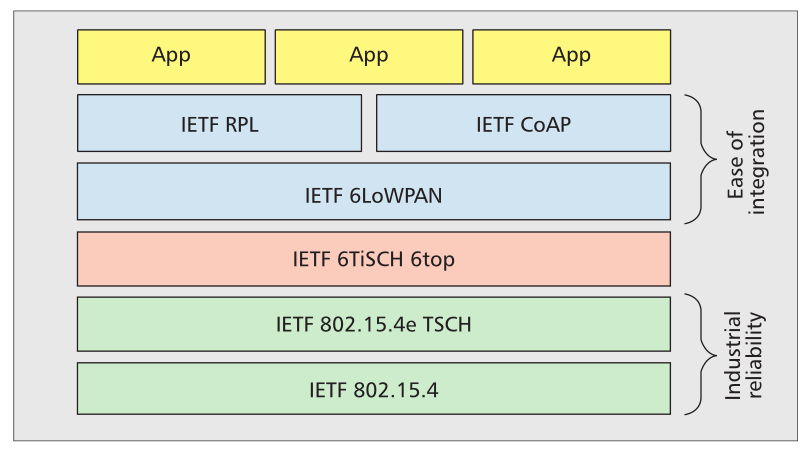
\includegraphics[width=1\linewidth]{pics/jaran}
	\caption{The protocol stack for the IIoT}
	\label{fig:jaran}
\end{figure}

\subsection{Congestion Control}

However, in a large-scale network, congestion becomes one of the significant problems which can prevent IIoT to work appropriately. Resource constraints, high traffic-load, and the high numbers of deployed sensors lead to network congestion \cite{GHAFFARI2015101}, which occurs when the transmitted packet load exceeds the available buffer capacity at any given time. This could lead the degradation of the network's quality of service (QoS), characterized by low throughput, long delay, and increased packet loss. Moreover, a harsh condition in the Industrial environment makes it prone to congestion. Hence, controlling congestion is a significant challenge in IIoT.

Due to the event-driven nature of WSNs, resource constraints, many-to-one communications, number of deployed sensors and the high traffic of sensor nodes lead to the creation of congestion in these networks. In WSNs, network congestion occurs when the offered traffic load exceeds the available capacity at any point in the network \cite{5760292}. Indeed, it can be mentioned that congestion is one of the highly critical challenges in WSNs and it has a profound impact on QoS parameters and the energy efficiency of sensor nodes. Moreover, congestion increases packet loss and degrades the throughput or wireless channels. Thus, to handle such challenges and problems in WSNs, researchers should consider and control the factor of congestion as shown in Fig. \ref{fig:gaktahu1}. 

\begin{figure}
	\centering
	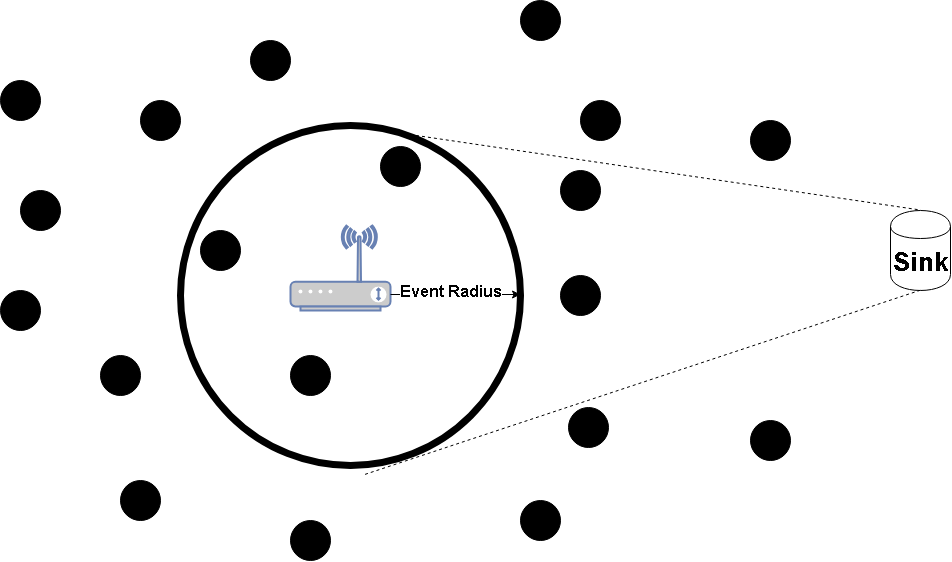
\includegraphics[width=1\linewidth]{pics/gaktahu1}
	\caption{Many-to-one data transmission scheme}
	\label{fig:gaktahu1}
\end{figure}


Fig. \ref{fig:gaktahu2} illustrates congestion in WSNs is created at two levels: node-level congestion (or buffer overflow) and link-level congestion. In node-level congestion, when packet arrival rate is higher than packet service rate, congestion is caused. This type of congestion occurs mostly in those sensor nodes which are closer to the sink.
Node-level congestion increases packet loss and power waste in WSNs. Consequently, this type of congestion has a direct impact on network availability and network lifetime. Factors such as competition, collision and bit error result in link-level congestion. Thus, in this kind of congestion, packet delivery rate in sink node is reduced. Therefore, for enhancing throughput and packet delivery rate at the sink node, collision should be prevented by using an appropriate medium access control based congestion control algorithms.

\begin{figure}
	\centering
	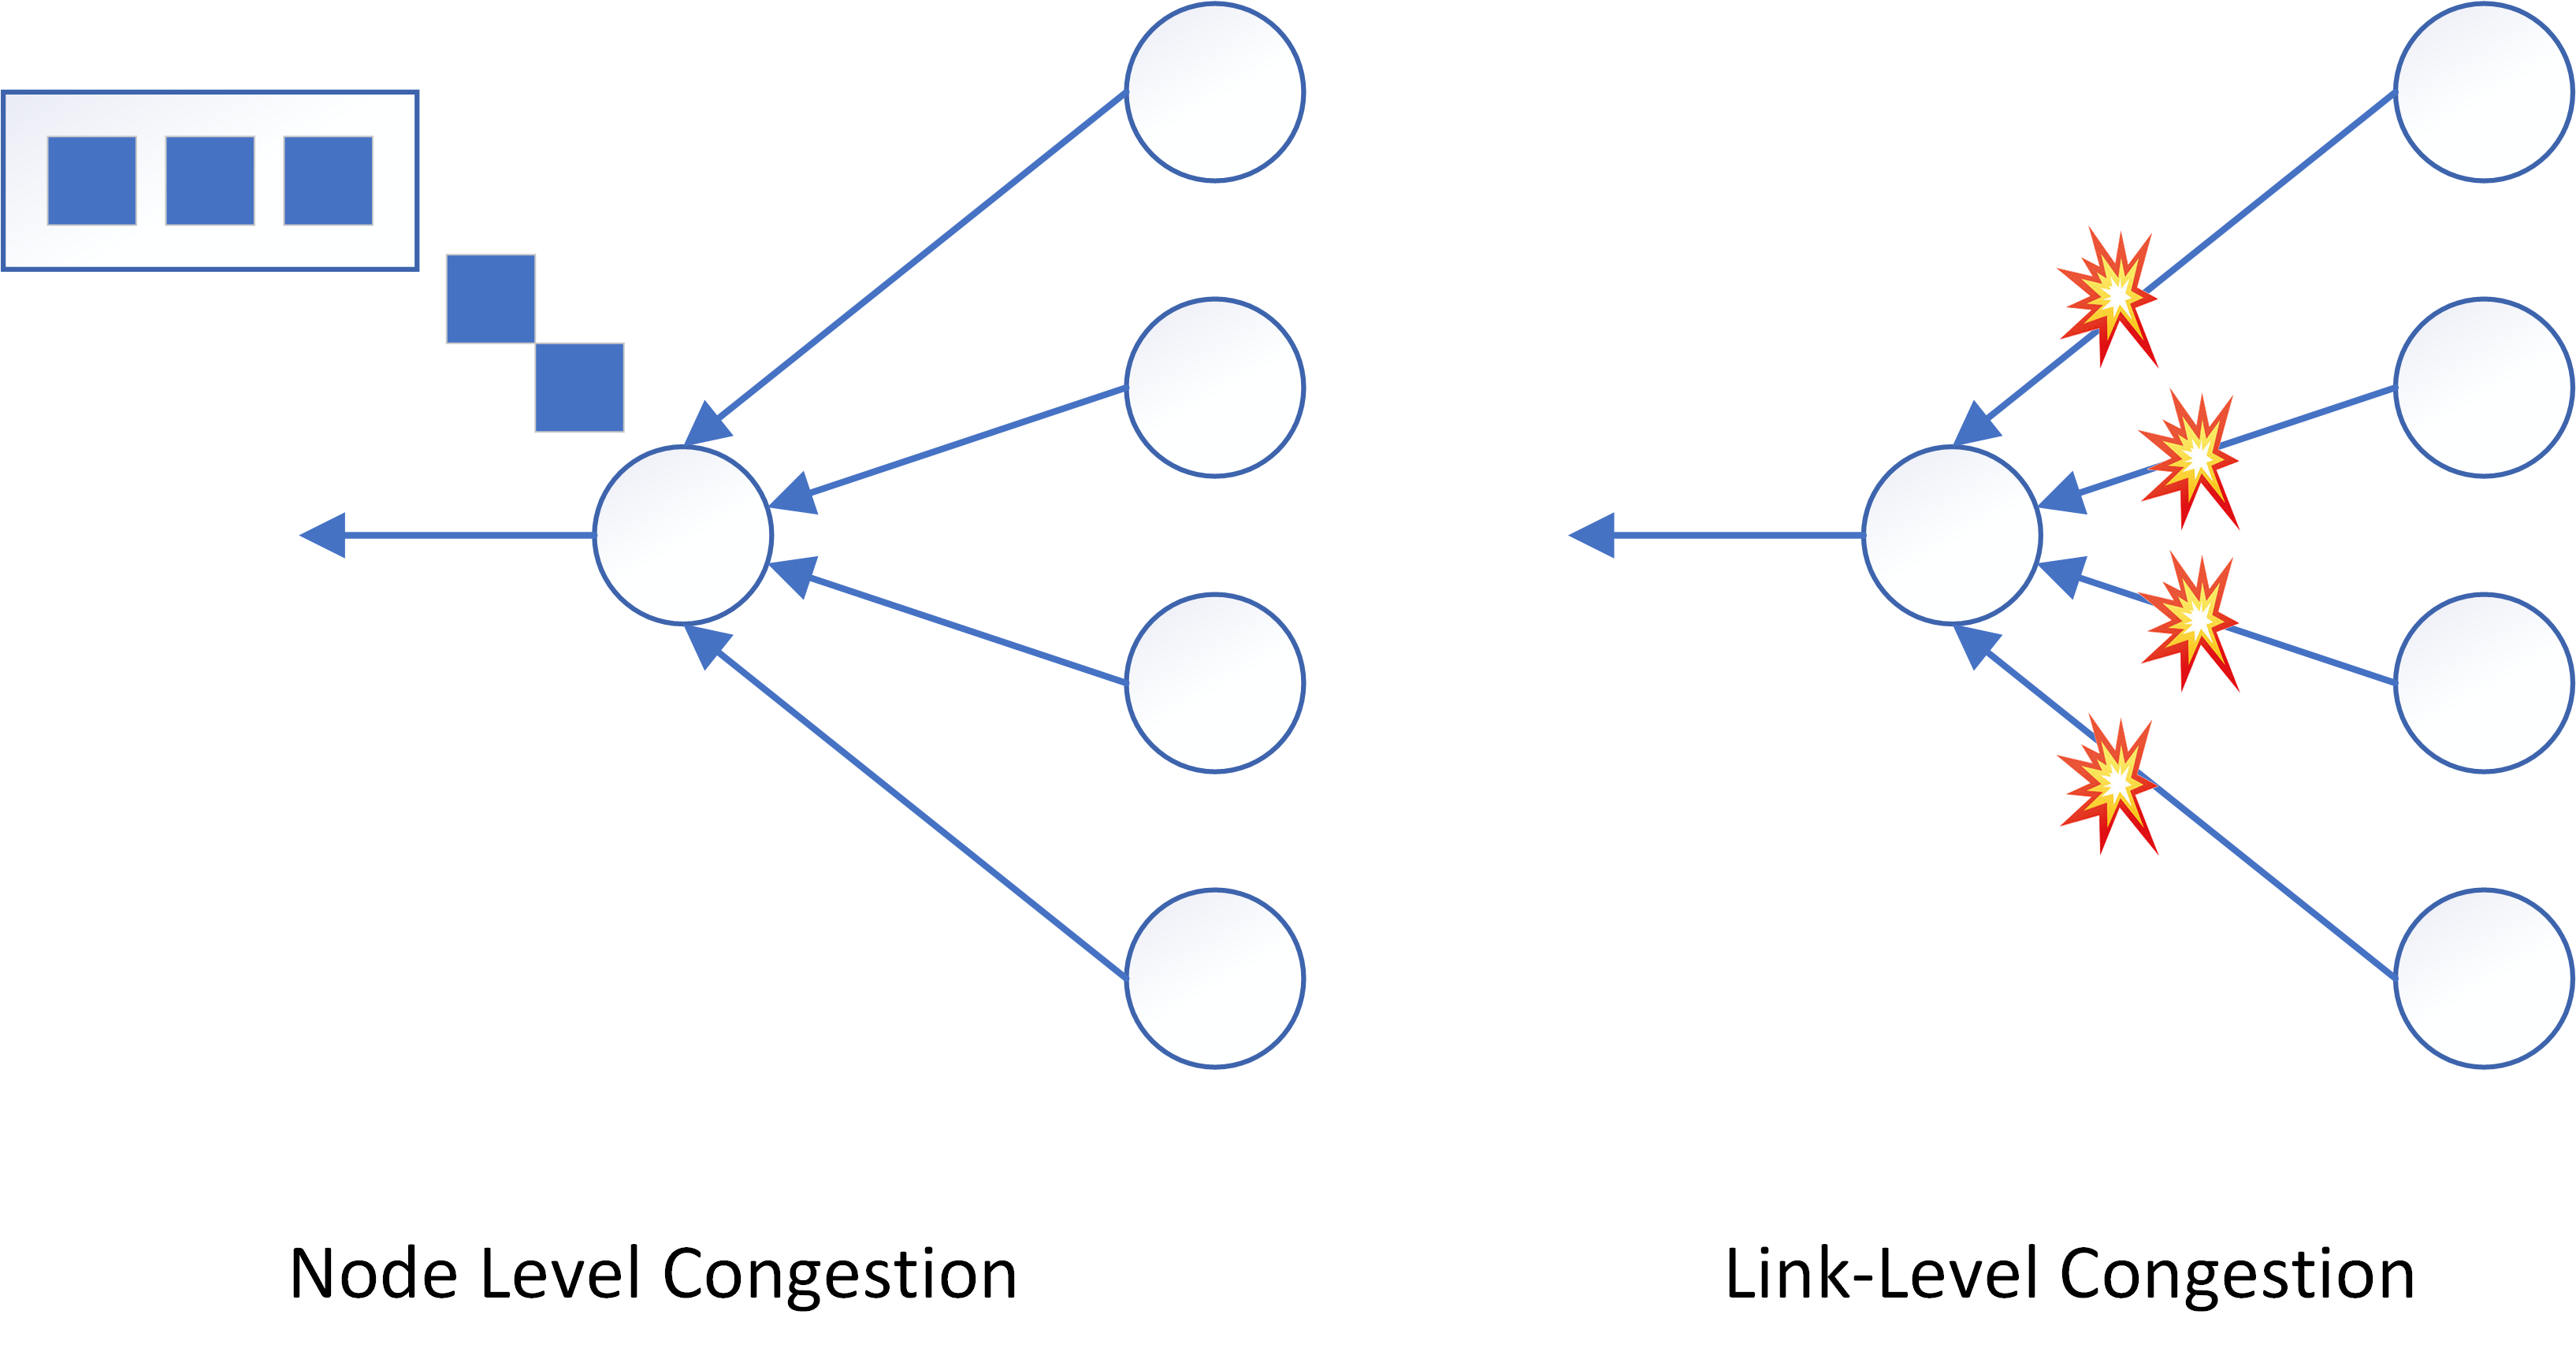
\includegraphics[width=1\linewidth]{pics/gaktahu2}
	\caption{Common congestion positions}
	\label{fig:gaktahu2}
\end{figure}


\section{Related Works}



The conventional method for mitigating congestion namely additive increase multiplicative decrease (AIMD) \cite{CHIU19891}. AIMD checks the available buffer capacity through slow enhancement of congestion detection condition. When congestion is detected, the protocol decreases the congestion window significantly. Through this scheme, congestion is reduced. However, AIMD provokes a saw-tooth-like rate which violates the QoS. Besides, AIMD scheme takes a long time for data rates to converge.

Woo et al. \cite{Woo:2001:TCS:381677.381699} introduced the Adaptive Rate Control protocol which was aimed at monitoring the injection of packets into the traffic stream as well as route-through traffic. In ARC, each node estimates the number of upstream nodes and the bandwidth is split proportionally between a relay and locally-generated traffic; however, the preference is given to the former. In ARC, in case an intermediate node overhears that the packets it sent previously are successfully forwarded again by its parent node, it will increase its rate by the constant $ \alpha$. Otherwise, it will multiply its rate by a factor $\beta$ where $0 < \beta <1$. ARC does not explicitly detect congestion and does not notify congestion explicitly; thus, it avoids using control messages. ARC improves fairness and is considered to be an energy-efficient congestion control algorithm for WSNs. However, it should be pointed out that ARC rate adjustment scheme introduces packet loss. 

Wan et al. \cite{Wan:2003:CCD:958491.958523} proposed congestion detection and avoidance (CODA) protocol for controlling congestion in WSNs. CODA amalgamated the present and past channel load and the level of buffer load to detect congestion at the intermediate sensor nodes. This protocol makes use of two strategies to control congestion: open-loop hop-by-hop backpressure and closed-loop multi-source traffic regulation. In open-loop hop-by-hop backpressure used for transient congestion, a node broadcasts back-pressure messages upstream towards source nodes to reduce their transmission rates. In closed-loop multi-source regulation which is based on end-to-end acknowledgment
and is used for persistent congestion, the sink asserts congestion control over many source nodes. To regulate data transmission rate, sink node transmits ACK packets towards nodes. In CODA, control packets such as ACK and backpressure consume the additional energy of the sensor nodes. CODA does not provide flow fairness and differentiates services into multiple classes of traffic. CODA adjusts rate through AIMD mechanism which often leads to packet loss. CODA carries out unidirectional congestion control, increases timelines but does not consider reliability. 

In congestion control and fairness (CCF) protocol \cite{Ee:2004:CCF:1031495.1031513}, congestion detection depends on packet service time, and every sensor node controls the rate of its downstream nodes. This method uses a scalable and distributed algorithm to conduct upstream congestion control which ensures the fair delivery of the packets to the central station as well as congestion elimination. CCF formulates congestion control and determines the number of downstream nodes, an average transmission rate of the packets and the production rate in each sensor. CCF precisely adapts traffic rate according to packet service time and fair packet scheduling algorithms. CCF controls congestion hop-by-hop, and each node uses precise rate adjustment based on available service rate and child node number. Rate adjustment in CCF is a function of packet service time which can result in low utilization when some sensor nodes do not have enough traffic or significant packet error rate. However, CCF does not take current queue utilization into account which results in the increased queuing delays, and various buffer overflows as well as increased retransmissions.

Hull et al. \cite{Hull:2004:MCW:1031495.1031512} introduced Fusion as a method for mitigating congestion; this method detects congestion through queue lengths. Moreover, Fusion makes use of hop-by-hop flow control, rate limitation and a prioritized MAC technique to handle congestion. If the packets of nodes are intended to be dropped downstream, hop-by-hop flow control stops them from transmitting packets because of insufficient buffer spaces. When compared with other uncongested nodes, it is observed that this priority is accomplished through decreasing the random back-off timer of congested nodes. Rate limitation metrics of traffic are accepted into a network to prevent unfairness towards sources located far from the sink. A prioritized CSMA-based MAC ensures that the congested nodes should receive prioritized access to the channel. As a result, it should be maintained that FUSION optimizes fairness and has a good throughput; nevertheless, it is only useful in case all nodes have the same traffic load \cite{8115774}. Moreover, fusion is not able to guarantee an optimal transmission rate for those nodes which are both fair and efficient.

Vedantham et al. \cite{1495018} proposed an adaptive, explicit rate control method, referred to as congestion control from sink to sensors (CONSISE). This method adjusts the downstream transmission rate at each of the sensor nodes to utilize the available network bandwidth. It should be noted that CONSISE is regarded as a highly scalable and easily implementable method which has remarkable performance advantages; that is, it uses resources efficiently with minimal overheads. In CONSISE, as
a node receives a packet from an upstream node, it will piggyback the respective information based on its current transmission rate and its node identifier. Moreover, as each downstream node receives a packet, it updates the information for the number of packets received from a specific node. At the expiry of a periodic timer, a node specifies its transmission rate and gives
explicit feedback to the upstream node. Scheuermann et al. \cite{Scheuermann:2008:IHC:1314716.1314991} put forth a hop-by-hop congestion control protocol designed for the unique features of the shared medium. This proposed congestion control protocol ensures that changing common conditions are replied rapidly and that the overhead is negligible. 

Yin et al. \cite{5164958} proposed Fairness-Aware Congestion Control (FACC) which is intended to control congestion and maintain approximately fair bandwidth allocation for different flows. Near-source nodes maintain a per-flow state and allocate an approximately fair rate to each passing flow. In contrast, near-sink nodes do not have to keep a per-flow state and use a lightweight probabilistic dropping algorithm according to queue occupancy and hit frequency. Indeed, it can be mentioned that FACC optimizes throughput, packet loss, energy efficiency and fairness. 

CADA. Fang et al. \cite{Fang2009} presented a scheme for congestion avoidance, detection and alleviation (CADA) in WSNs. This scheme optimizes energy consumption and information loss problems. By exploiting data features, a few representative sensor nodes are selected from those in the event area as data sources: as a result, source traffic can be mitigated and controlled pro-actively. Consequently, the potential congestion is avoided. When congestion takes place unavoidably as a result of traffic emergency, it will be detected immediately by the hot spot node based on a combination of buffer occupancy and channel utilization. Moreover, congestion is alleviated reactively by either dynamic traffic control or source rate regulation according to specific hot spot scenarios. In other words, it can be mentioned that CADA optimizes throughput, energy consumption, and average end-to-end delay.

Enhanced congestion detection and avoidance (ECODA) was developed to use dual buffer thresholds and weighted buffer difference for detecting congestion in WSNs \cite{5606274}. ECODA includes three mechanisms: (1) in the first strategy, dual buffer thresholds and weighted buffer difference are used as to detect congestion; (2) the second strategy makes use of flexible queue scheduler based on packet priority; (3) the control scheme of bottleneck node-based source transmission rate is used as the third strategy in case of persistent congestion. Indeed, ECODA uses hop-by-hop congestion control
scheme for transient congestion. Brahma et al. \cite{BRAHMA2012670} put forth a distributed congestion control algorithm for tree-based communications in WSNs; this algorithm assigns a fair and efficient transmission rate to each node. Also, each node controls and monitors its aggregate output and input
traffic rate. For the difference between input and output traffic rate, a node decides on whether to increase or decrease the bandwidth; such a decision to increase or decrease
the bandwidth is allocated to the flow that originates from itself and its neighboring nodes.

Domingo et al. \cite{DOMINGO2013203} introduced bio-inspired congestion control for underwater WSNs. This algorithm differentiates packet losses due to congestion from packet losses related to high link error rates. It provides flow fairness, but it does not guarantee reliability which is vital in IIoT.

A recent bio-inspired congestion control scheme was introduced that mimics the flocking of birds \cite{ANTONIOU20131167}. Bird behavior was used as a basis to design a robust, scalable, and decentralized congestion control scheme for WSNs. By moving packets to the sink and exploiting available network resources, the load is balanced. Moreover, flock-CC can reduce packet loss with various traffic load conditions. However, this scheme does not address fairness since not all sensor nodes can have same chance to transmit their packet load.

Previous work on congestion control involving mathematical models of population biology was proposed for the Internet by either improving the current TCP CC mechanism \cite{Analoui:2006:CFB:1315843.1315889} or providing a new way of combating congestion \cite{Hasegawa:2006:TSC:1190326.1190338}. The study of \cite{Analoui:2006:CFB:1315843.1315889} couples the interaction of Internet entities that are involved in CC mechanisms (routers, hosts) with the predator-prey interaction. This model exhibits fairness and acceptable throughput but slow adaptation to traffic demand. Recent work by Hasegawa et al. \cite{Hasegawa:2006:TSC:1190326.1190338} focuses on a new TCP CC mechanism based on the LV competition model which is applied to the congestion window updating mechanism of TCP. According to the authors, remarkable results regarding stability, convergence speed, fairness, and scalability are exhibited. However, these approaches are based on the end-to-end model of the Internet.

\section{Motivation and Contributions}

In this thesis, a hybrid of two bio-inspired algorithms for congestion control is investigated. The first one is a competitive Lotka-Volterra (C-LV) model \cite{pop00001, NGUYEN20171192}. By using C-LV, congestion avoidance can be guaranteed. It is a decentralized scheme that controls the rate of transmission to prevent congestion while achieving fairness among all sensor nodes. The primary objective of using C-LV is to provide efficient and smooth rate adaptation while avoiding congestion in traffic and maintaining fairness. C-LV provide a coexistence solution by adequately choosing the parameters to guarantee congestion-free traffic. However, appropriately choosing parameters could be time-consuming and seemingly impossible if there is an enormous number of nodes. To address this problem the second bio-inspired algorithm in this thesis is introduced.

The second proposed algorithm is the dragonfly algorithm (DA) \cite{Mirjalili2016}. In the C-LV model, there are critical parameters that must be appropriately chosen. DA can be employed to carry out this task. In addition to avoiding congestion and maintaining fairness, DA enhances the C-LV scheme by optimizing the transmission rate. With throughput as the objective function of DA, agents find a solution with the objective of minimizing delay as much as possible. Unlike gradient descent, DA is not prone to be trapped in a local optimum solution and has a high chance achieving a global optimum solution. By combining these two algorithms, congestion-free traffic with fairness and the lowest possible end-to-end delay is achieved without the need to choose critical parameters manually. 

The contributions of this thesis are summarized as follows:
\begin{enumerate}
	\item Hybrid bio-inspired algorithms for congestion control in large-scale IIoT are introduced.
	\item Due to the decentralized nature of the scheme, the overhead is minimized.
	\item The C-LV scheme guarantees congestion-free traffic and maintains fairness for each sensor node.
	\item The DA enhances the C-LV model by providing an optimal parameter for minimizing end-to-end delay as much as possible.
	\item The adaptive nature of the scheme helps the system to adapt to changes such as an increased or decreased number of the sensor nodes during operation.
\end{enumerate}

The simulation results verify that the proposed scheme guarantees congestion-free traffic and maintains fairness among sensor nodes.  A packet load is transmitted as fast as possible without causing congestion. Moreover, the simulation results demonstrate the adaptiveness of the scheme in responding to dynamic change.

The remainder of this thesis is organized as follows. In Chapter II, the overview of C-LV and DA is presented in detail, and the proposed Bio-inspired congestion control mechanism for IIoT is elaborated. In Chapter III, the simulation results are presented. Finally, Chapter IV presents the conclusions and directions for future work.